\subsubsection{Model Representation}
\begin{itemize}[--]
	\item Goal is model labelled data (data which we have the correct output for) to a line 
	\item Notation:\begin{description}
		\item[$m$] = number of training examples
		\item[$x$] = input variable/feature
		\item[$y$] = output variable/feature
		\item[$(x,y)$] = one training example
		\item[$(x^{(i)},y^{(i)})$] = $i$th training example (parens indicate index)
	\end{description}

	\item We take a training set, input into a learning algorithm, which returns a hypothesis ($h$) that models the relationship.
	\begin{center}\begin{tikzpicture}[node distance = 2cm, auto]
		%Place nodes
		\node [block] (train) {Training Set};
		\node [block, below of=train] (alg) {Learning Algorithm};
		\node [block, below of=alg] (hyp) {$h$};
		\node [cloud, left of=hyp] (x) {$x$};
		\node [cloud, right of=hyp] (y) {$y$};

		%Draw edges
		\path [line] (train) -- (alg);
		\path [line] (alg) -- (hyp);
		\path [line] (x) -- (hyp);
		\path [line] (hyp) -- (y);
	\end{tikzpicture}\end{center}
	\item $h$ maps from $x$'s to $y$'s ($h(x)=y$).
	\item We need to determine how we want to represent $h$
	\item A simple linear model with one variable for $h$ is: $$h_\theta (x) = \theta_0 + \theta_1 x$$, called \textbf{univariate linear regression}.
\end{itemize}

\subsubsection{Cost Function}
\begin{itemize}[--]
	\item Given a hypothesis: $h_\theta (x) = \theta_0 + \theta_1 x$
	\begin{description}
		\item[$\theta_i's$] = parameters of the model
	\end{description}

	\item We will now discuss how to choose the parameters of our model
	\item Idea: choose $\theta_0, \theta_1$ so that $h_\theta (x)$ is close to $y$ for our training examples $(x,y)$
	\item We want to minimize $\theta_0, \theta_1$ such that $h(x) - y$ is minimal (reminder: $h(x)$ is the guess at the correct value at $y$).
	\item Because we we only are looking to minimize our absolute distance, we square the distance we want to minimize to account for positive and negative differences equally now making our cost function: $(h(x)-y)^2$
	\item However, we don't want to minimize it for just one example, so we do this for every training example: $$\sum_{i=1}^{m}(h_\theta (x^{(i)}) - y^{(i)})^2$$
	\item To make later math easier, we further refine our formula to be half the average: $$\frac{1}{2m}\sum_{i=1}^{m}(h_\theta (x^{(i)}) - y^{(i)})^2$$
	\item This function we created is called our \textbf{cost} function, as it measures how expensively incorrect our current model is, which we will denote with $J$. 
	\item The cost function is dependent on the hypothesis parameters, and our goal is to adjust these parameters to minimize the overrall cost of our model: $$J(\theta_0, \theta_1) = \frac{1}{2m}\sum_{i=1}^{m}(h_\theta (x^{(i)}) - y^{(i)})^2$$
	\item Now our goal is to minimize $J$ over the variables $\theta_0, \theta_1$
\end{itemize}

\subsubsection{Cost Function - Intuition I}
\begin{center}
	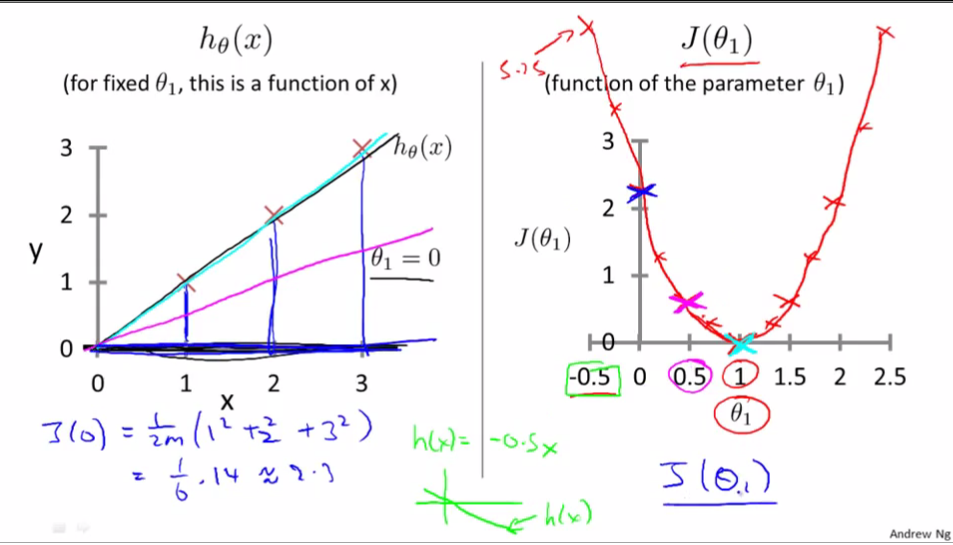
\includegraphics[scale=0.75]{sections/cs229/w1/cost_function.png}
\end{center}
This image shows that for varying parameter values, the cost function changes. In this idealistic example there's a global minimum, the goal of minimized cost, that is very easily followed by a hill-climbing style algorithm.

\subsubsection{Cost Function - Intuition II}
\begin{center}
	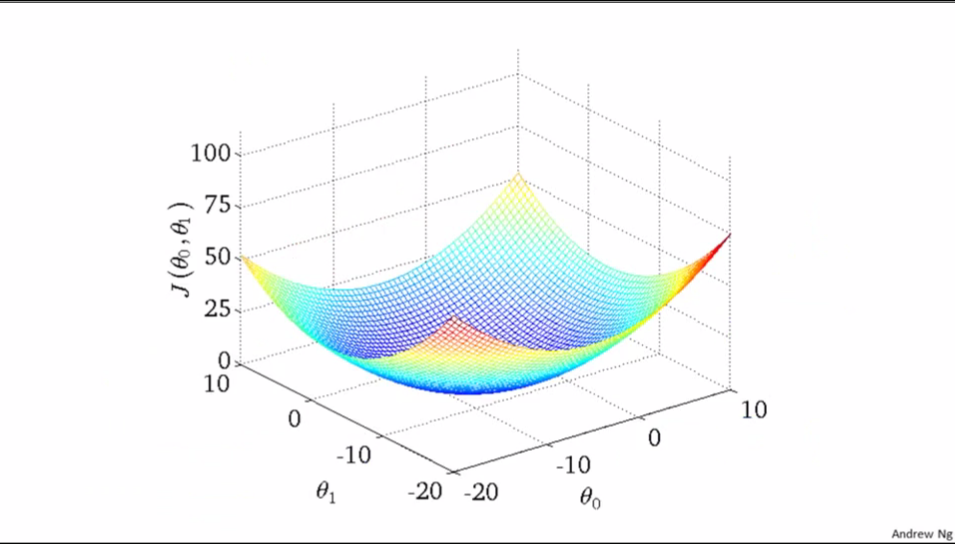
\includegraphics[scale=0.75]{sections/cs229/w1/2d_cost_function.png}
\end{center}
Similarly when you have an additional variable, you want to reach the bottom of this $N$-dimensional hill (note: not all models will have such a perfect hill). 
\begin{itemize}[--]
	\item The gradient gives the direction of maximumal increase on a surface.
	\item We will use a negative gradient to find the `direction' to travel towards the bottom of the hill
	\item Another common way to represent multidimensional cost functions is through contour plots
	\item 
\end{itemize}

\subsubsection{Gradient Descent}
\begin{itemize}[--]
	\item Given some function $J(\theta_0, \theta_1,\ldots ,\theta_n)$ we want to minimize $J$ with respect to $\theta_0, \theta-1,\ldots ,\theta_n$. 
	\item Choose initialize values for the parameters (eg. $\theta_0=\ldots=\theta_n =0$)
	\item Iteratively change $\theta_0, \ldots, \theta_n$ to reduce $J(\theta_0, \ldots, \theta_n )$, until hopefully a minimum is achieved.
	$$\theta_j := \theta_j - \alpha \frac{\partial}{\partial \theta_j}J(\theta_0,\ldots, \theta_n)$$
	\item $\alpha$ is the learning rate, which determines how much change happens in each update
 	\item Ensure simultaneous update, store in temps and then assign.
	\item An issue with gradient descent is finding local minimums, because you won't be able to find the optimal solution. 
	\item 
\end{itemize}

\subsubsection{Gradient Descent Intuition}
\begin{itemize}[--]
	\item To simplify, we will consider the cost funciton with 1 variable ($J(\theta_0)$).
	\item The negative gradient means that you negative slope, which results in increases with negative slope and dcreases with positive slopes
	\item If $\alpha$ is too small, gradient descent can be very slow.
	\begin{center}
		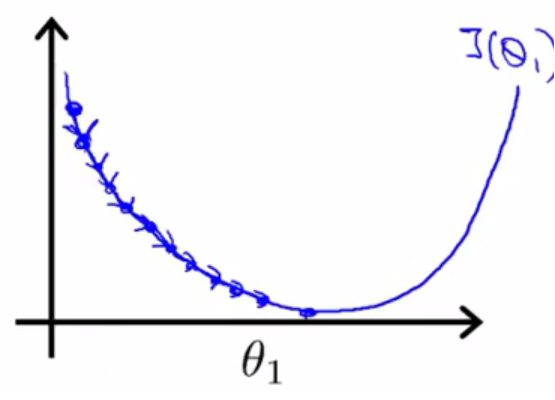
\includegraphics[scale=0.75]{sections/cs229/w1/alpha_small.png}
	\end{center}

	\item If $\alpha$ is too large, it may fail to converge (not reach minimum).
	\begin{center}
		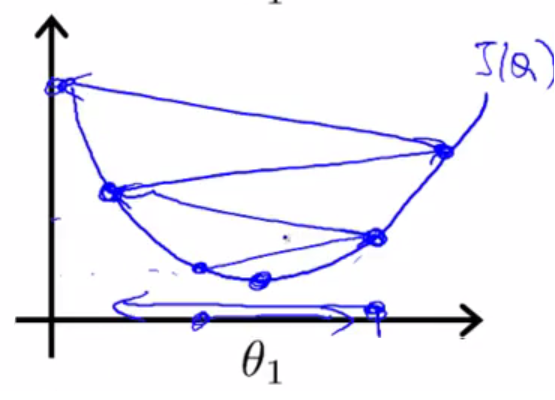
\includegraphics[scale=0.75]{sections/cs229/w1/alpha_large.png}
	\end{center}

	\item If you're already at the local minimum, you will not change your parameters because the gradient is zero.
	\item You can still converge to a local minimum with a fixed $\alpha$ (learning rate) because as we approach the minimun the gradient descent will automatically take smaller steps.
	\item 

\end{itemize}